
\chapter{Vertical betatron oscillations} % Main chapter title
\label{Chapter6} % For referencing the chapter elsewhere, use \ref{Chapter6} 

\section{Introduction}

The muon g-2 storage ring acts as a weak focusing betatron. The experiment uses quadrupoles held at an adjustable voltage. The electric field provided by the quadrupoles gives a linear restoring force in the vertical direction, focusing the beam vertically but defocusing radially. However, the combination of the vertical dipole magnetic field and the defocusing radial electric field provides a net linear restoring force in the radial direction and so the beam is focused in both directions. The E-field and the B-field determine the dispersion of the beam and the $\beta$-functions, the measurements of which will be the focus of this chapter.

The muons that enter the ring have to pass through the inflector, which is an aperture vertically $\sim{15}$ cm and radially $\sim{7}$ cm wide. These muons do not all have the magic momentum and so the beam has a momentum spread. The restoring forces from the two fields cause the muons to oscillate about an equilibrium position. Vertically, for ideal quadrupoles, the equilibrium position $y_{e}$ is at the centre of the storage ring $(y = 0)$. The radial equilibrium position $x_{e}$ is determined by the muons momenta. This leads to both the average position and width of the muon beam to exhibit simple harmonic motion called betatron oscillations, in both the radial and vertical directions. 

The equations for the horizontal and vertical beam motion are given by 
\begin{equation}
x = x_{e} + A_{x}\mathrm{cos}(v_{x}\frac{s}{R_{0}} + \delta_{x}),
\end{equation}
\begin{equation}
y = y_{e} + A_{y}cos(v_{y}\frac{s}{R_{0}} + \delta_{y}),
\end{equation}

\noindent
where $\nu_{x}$ and $\nu_{y}$ are the horizontal and radial beam tunes respectively, s is the arc length along the trajectory, $R_{0}$ is the magic radius and $\delta_{x}$ and $\delta_{y}$ are the corresponding phases. The tune is defined to be the number of betatron oscillations per revolution of the storage ring and is related to the strength of the field, characterised by the field index n. The field index is given by:

\begin{equation}
n=\frac{{\kappa}R_{0}}{{\beta}B_{0}}
\end{equation}

\noindent
where $\kappa$ is the electric quadrupole gradient, $R_{0}$ = 7112mm which is the radius of the storage ring, $\beta$ is the relativistic velocity of the muon and $B_{0}$ is the magnetic field strength. The corresponding tunes are:

\begin{equation}
v_{x} = {\sqrt{1-n}},
\end{equation}
\begin{equation}
v_{y} = \sqrt{n}.
\end{equation}

To go from the tunes to the oscillation frequencies we multiply by the cyclotron frequency $f_{c}$. For the initial running conditions the quadrupoles were set to $18.3$ kV during data taking, giving a corresponding field index of $n = 0.108$. The resulting horizontal and vertical betatron frequencies are:

\begin{equation}
{f_{x} = f_{c}\sqrt{1-n} \simeq 0.94f_{c}} = 6298\mathrm{ kHz},
\end{equation}
\begin{equation}
{f_{y} = f_{c}\sqrt{n} \simeq 0.33f_{c}} = 2211\mathrm{ kHz}.
\end{equation}

\subsection{The effect of betatron oscillations on $\omega_{a}$}

Precise knowledge of the muon beam distribution and its behaviour throughout the fill is required to determine the corrections needed to calculate $a_{\mu}$. This is because as the beam undergoes these radial and vertical oscillations the rate of positrons measured by the detectors, which have an acceptance that depends upon the decay position, also oscillates. Thus the total number of detected positrons will vary throughout the fill due to the oscillation of the centroid of the beam distribution, as well as due to the precession of the muon spin and the width. The simple 5 parameter fit function used to fit $\omega_{a}$ is 

\begin{equation}
N(t)_{5par} = N_{0}e^{-\frac{t}{\gamma\tau}}(1+A\mathrm{cos}(\omega_{a}t + \phi))
\end{equation}

\noindent 
Where $N_{0}$ is an estimate of the number of muons at start time, $\gamma\tau$ is the average relativistic lifetime of the stored muons, A is the amplitude of the precession oscillation (asymmetry term) and $\phi$ is the phase of precession at the start time. This is modified to account for the variation in the positron rate due to the betatron oscillations by:

\begin{equation}
N(t) = N(t)_{5par}\cdot{N_{CBO}}(t),
\end{equation}
\noindent
with
\begin{equation}
{N_{CBO}}(t) = 1 + A_{CBO}\mathrm{cos}(\omega_{CBO}t) + \phi_{CBO})e^{-\frac{t}{\tau_{CBO}}}
\end{equation}

\noindent
Where $A_{CBO}$ is the amplitude of the CBO, $\omega_{CBO}$ is the frequency of the CBO term, $\phi_{CBO}$ is the phase of the CBO at the start time and $\tau_{CBO}$ is the lifetime of the CBO. The general form for an oscillation term is an exponentially decaying sinusoid. One such term is added for all the observed betatron oscillations. As well as directly affecting N, there are effects from the betatron oscillations on the phase and amplitude in the final $\omega_{a}$ fits. 

\begin{equation}
{A}(t) = 1 + A_{A}\mathrm{cos}(\omega_{CBO}t + \phi_{A})e^{-{\frac{t}{\tau_{CBO}}}}
\end{equation}

\begin{equation}
{\phi}(t) = 1 + A_{\phi}\mathrm{cos}(\omega_{CBO}t + \phi_{\phi})e^{-{\frac{t}{\tau_{CBO}}}}
\end{equation}

\noindent
Here we have moved from A and $\phi$ defined in equation 7.8 to time dependant A and $\phi$, where $A_{A}$ and $\phi_{A}$ refer to the amplitude and phase of the CBO oscillation in the asymmetry term and $A_{\phi}$ and $\phi_{\phi}$ are the amplitude and phase of the CBO oscillation of the $\phi$ term. The relevant betatron oscillations for the run 1 dataset are defined later in this chapter. In order to minimise the impact of these oscillations on the $a_{\mu}$ measurement tuning is required in order to ensure that the betatron wavelengths are not multiples of the storage ring circumference. If the beam after one full rotation around the ring is situated back in the same exact position then the beam would sample the magnetic field at the same position each time. Any deviations in the magnetic field and quadrupole electric fields will lead to forces that affect the muons orbit with each revolution of the ring. If these forces lie on a resonance then the betatron oscillations will increase and could cause muon loss. Any imperfections in the magnetic field would lead to these field errors accumulating each revolution. Instead the tune is used to ensure that the beam is at a different position every revolution, for example a muon travels a bit more than a full revolution until it gets back to the same radial position ensuring that the beam samples the whole magnetic field across the azimuth. 

The equations used to describe the beam oscillations assume uniform coverage of the quadrupoles. However in the experiment only 43$\%$ of the storage ring is covered by the quadrupoles and therefore the equations are only approximate. The focusing strength will change as a function of azimuth around the ring and a measurement of the beam dynamics at different azimuthal positions is required.

\subsection{Coherent betatron oscillations}

Each stationary tracking detector only observes the beam from one position around the ring and therefore only measures the beam once for each revolution of the storage ring (cyclotron period). This means that only frequencies of less than 0.5 $f_{c}$ can be observed. When considering the radial width, it is narrow at injection into the storage ring as the entrance is oval shaped; long vertically and narrow radially. Due to the tuning, each muon does not complete a full oscillation until it has done more than one rotation around the ring. This means that the focal point as measured by a stationary detector from injection will move azimuthally during the fill and the width will swim around the ring as the muons orbit it. Furthermore there is an additional focal point at a time of half a betatron period due to the sinusoidal nature of the muons radial position.
The ranges of the field index n used by the experiment mean that the radial beam oscillation frequency is higher than the vertical oscillation. The radial oscillation $f_{x}$ > 0.5$f_{c}$ and so instead of observing the true frequency an aliased frequency is measured at a frequency of $f_{CBO}$ = $f_{c}$ - $f_{x}$, which is determined from the Nyquist theorem. The frequency of this is called the Coherent Betatron Oscillation $f_{CBO}$. 
The frequency at which a single fixed detector sees the beam coherently moving back and forth radially is given by

\begin{equation}
f_{CBO} = f_{C} - f_{x} = (1 - \sqrt{1-n})f_{C}
\end{equation}
So the oscillation of the radial mean is measured at a lower aliased frequency of $f_{CBO}$ while the vertical oscillation which has a frequency $f_{y}$ < 0.5$f_{c}$ is measured at its actual frequency. A diagram illustrating this is shown in figure 7.1. From this diagram it can also be seen that the oscillation at twice the vertical mean oscillation, which corresponds to the vertical width of the beam, is aliased. The measured frequency will be: 

\begin{equation}
f_{VW} = f_{C} - 2f_{y} = (1 - \sqrt{n})f_{C}
\end{equation}
\noindent
Where the $f_{VW}$ refers to the frequency of the vertical waist, the term used to describe the vertical width of the beam.

\begin{figure}[th]
\centering
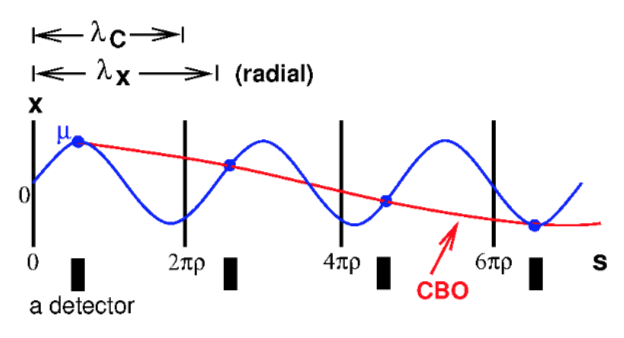
\includegraphics[scale=1.0]{Figures/CBOdiagram.png}
\decoRule
\caption{ An illustration of the coherent betatron oscillation (CBO). Showing in blue the radial betatron oscillation for several wavelengths. In black is the cyclotron circumference. As the radial betatron oscillation has a wavelength longer than the storage ring circumference the detector observes the muon beam to be moving closer to it and then move furher away. The frequency that the detector samples this beam motion is the CBO frequency.\cite{Reference29}}
\label{fig:CBOdiagram}
\end{figure}
Figures 7.2 and 7.3 give illustrations of the field index and frequency range that is affected by the aliasing effect for a detector at a fixed azimuthal position. 

\begin{figure}[!h]
\centering 
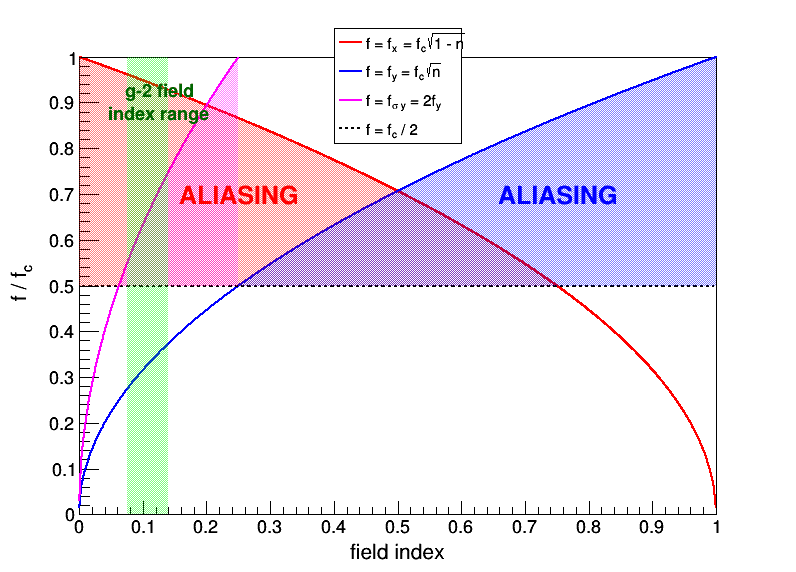
\includegraphics[scale=0.5]{Figures/freq_vs_n.png}
\decoRule
\caption{For a range of field indices (green shows those accessible for our experiment) it plots the frequency, and then also the Nyquist band, at $f_{c}$/2, above which we are aliased. The detectors can only measure frequencies less than half the $f_{c}$, so aliasing occurs at frequencies above this. The range of field indices which are determined by the strength of the quadrupoles is shown in green, and as seen the radial frequency will always be aliased.}
\label{fig:freq_vs_n.png}
\end{figure}

\begin{figure}[!h]
\centering 
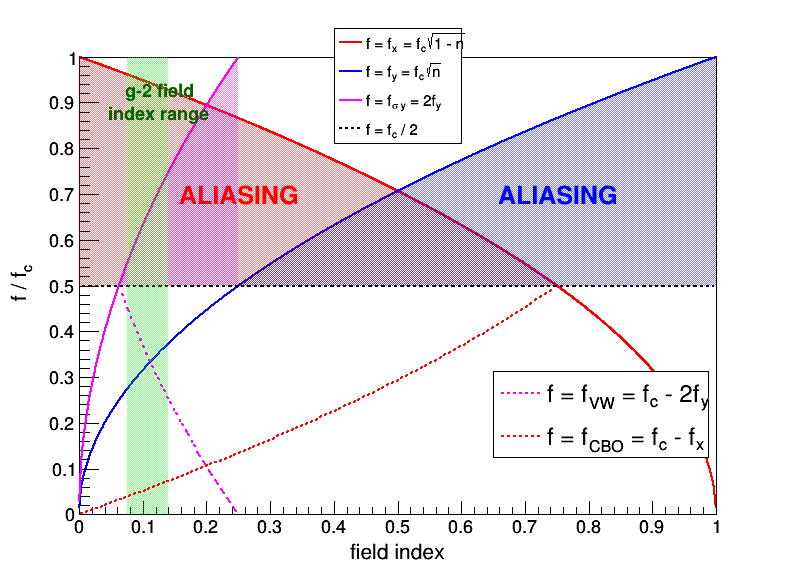
\includegraphics[scale=0.5]{Figures/freq_vs_n_alias.png}
\decoRule
\caption{Same plot but with the aliased frequency drawn on.}
\label{fig:freq_vs_n_alias.png}
\end{figure}

The calorimeter detector acceptance is dependant on the radial and vertical position of the muons decay. The muon beam distribution oscillates during the fill which will cause the rate of positrons measured to oscillate due to detector acceptance. This shows up as an amplitude modulation of the decay positron time spectrum data, and is accounted for using the equation 3.18. Any change in the betatron frequencies during the fill results in a systematic error on the $\omega_{a}$ measurement. The betatron frequencies themselves have frequencies much larger that $f_{a}$ and so do not affect the $\omega_{a}$ measurement directly. However the CBO frequency is close to the second harmonic of the $\omega_{a}$ frequency. The CBO causes issues with detecting $\omega_{a}$ when its frequency lies close to a multiple of $f_{a}$ or one of its side bands is close to $f_{a}$. For the 2000 run at BNL the $f_{CBO}$ did in fact lie close to the second harmonic of $f_{a}$ and affected the $\omega_{a}$ determined from fits of the data. This has been avoided for this experiment by selecting the right field strength. The quadrupole voltages that the experiment was ran at for run 1 were 18.3 kV and 20.4 kV.

Care must be taken when choosing the operating quadrupole voltage. This is because if the linear combination of both betatron frequencies is an integer of the cyclotron frequency then this can cause resonances. This would lead to the beam distribution expanding and therefore loss of muons. Spin resonances could also occur. This is where the spin is slightly rotated with each betatron cycle. These effects will slowly add up and lead to phase change of the $\omega_{a}$ oscillation, affecting its measurement.

\subsection{Lost muons}

Muons at the outer limits of the storage radius have a higher likelihood of being lost at early times. The muons which leave the storage region before decay are referred to as lost muons. These cause a deviation in the muon exponential decay curve, which affects the $\omega_{a}$ fits and leads to a shift in the $\omega_{a}$ calculated. Muons which lie on the outer edge of the muon beam distribution and are outside of the storage ring radius are removed by a process called scraping. This is where an asymmetric charge is placed on the electrostatic quadrupoles at early times causing the centroid of the beam to move radially and vertically by $\sim{2}$ mm, forcing the muons at the edge of the distribution into the path of collimators. This causes those muons to scatter, curl inwards and leave the storage ring \cite{muonloss1}. The quadrupoles are then restored to their nominal values and the remaining muons are stored. The vertical displacement of the muon beam distribution measured by the tracking stations over the course of the scraping period is shown in Figure 7.4. The binning chosen here was larger than the period of the expected oscillations so that only the effect of scraping can be seen. The $\omega_{a}$ fits do not start until 30 $\mu$s so that the effects of scraping are no longer present and the muon beam and corresponding betatron oscillations are constant throughout the fitting range.

\begin{figure}[!h]
\centering 
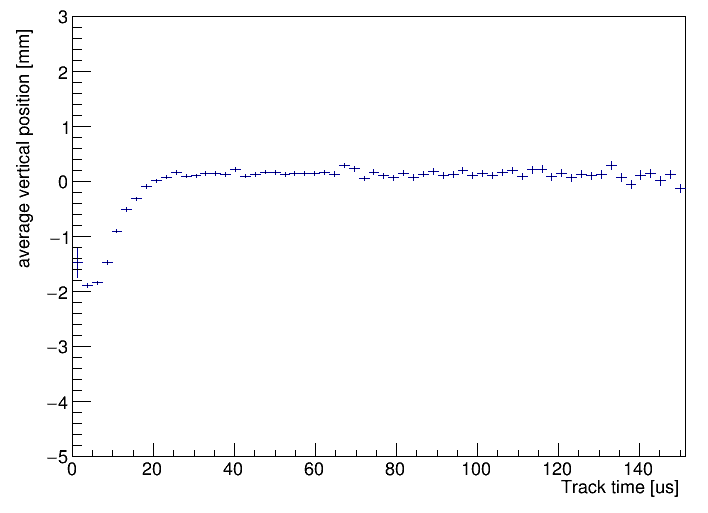
\includegraphics[scale=0.5]{Figures/AverageVerticalPosition_station12.png}
\decoRule
\caption{Measurement of the vertical displacement of the muon beam centroid at tracking station 12 during the scraping period.}
\label{fig:AverageVerticalPosition_station12}
\end{figure}

However a small amount of muons will continue to be lost at later times. This could be due to perturbations in the storage rings magnetic and electric fields or by scattering with residual gas in the storage ring with the radial and vertical betatron oscillations of the beam distribution also adding to this. When these muons are eventually lost they curl inwards and are capable of travelling through several calorimeters. They are therefore identified by double or triple coincidences with neighbouring calorimeters. The muon candidates are identified by depositing approximately 180 MeV into a calorimeter crystal. They are also more likely to just produce a signal in one crystal in the calorimeter as they are much less ionising that the positrons which are likely to deposit energy in several crystals as they pass through. The coincident muons in neighbouring calorimeters are determined by a signal time window with a time of flight of 6.25$\pm$0.5 ns \cite{muonloss2} for each adjacent calorimeter. These lost muon candidates can also be cross checked with the tracking detector information.

\section{Corrections to $\omega_{a}$ measurement}

After accounting for the lost muons $\omega_{a}$ is extracted from the calorimeter data. There are two additional corrections that need to be applied, due to beam related effects, the so called E-field and pitch corrections. As mentioned in chapter 3, the storage ring muons are chosen to be at the magic momentum and as such the quadrupole electric field does not affect $\omega_{a}$ directly. However corrections are required to account for muons not at the magic momentum (E-field correction) or not travelling perfectly perpendicular to the magnetic field (pitch correction). The size of the corrections are expected to be of order 450 and 200 ppb respectively, with a targeted combined uncertainty <50 ppb.  

\subsection{Radial electric field corrections}

The muon beam distribution is dependant on the phase space acceptance of the beam injection point at the inflector, the storage ring itself and the kick provided by the kicker to place the beam into the magic storage radius. As explained in chapter 3 $\omega_{a}$ is not affected by the electric field for muons at the 'magic' momentum of 3.09 GeV/c. However the storage ring momentum acceptance is $\pm{0.15}\%$ \cite{Reference29} and so there is a range of muon momenta around this magic momentum. Therefore the effect of the radial electric field cannot be completely ignored and will cause a systematic error in the $\omega_{a}$ value determined. To determine the correction required for the electric field the equilibrium radial distribution of the moun beam is required. This can be measured by analysing how the bunch structure evolves during the fill, a so called fast rotation analysis. For a beam with a range of momenta, the beam will undergo debunching. This is where muons with higher momentum will have the largest orbits and so will take the longest time to travel once around the ring while the lowest momentum muons will take the lower orbit and so complete one cycle around the storage ring in a shorter time than the higher momentum muons. Eventually after many cycles around the ring the low momentum muons will overtake the high momentum muons and will do so multiple times as the muon beam circulates the storage ring. This leads to a stretching of the muon bunch structure until the beam becomes uniform and the bunch structure is lost. The bunch structure has mostly disappeared by 60$\mu$s \cite{FR2}. 
The fast rotation analysis is carried out using calorimeter data. In the 2001 BNL data set, the electric field correction for the low n-value data set was +0.47 $\pm$ 0.05 ppm \cite{Reference13}.

\subsection{Pitch correction}

The measured $\omega_{a}$ value requires a correction due to the betatron oscillations having a small effect on $\omega_{s}$. In equation 3.15 it was assumed that the muon beams velocity is perpendicular to the magnetic field, thus the equation is simplified by the assumption that $B\cdot\beta$ = 0. However this is an approximation and for the high level of precision required for the $\omega_{a}$ measurement a correction is needed to account for the vertical betatron oscillations, where the muons velocity is not exactly perpendicular to the storage ring magnetic field.

\begin{figure}[!h]
\centering 
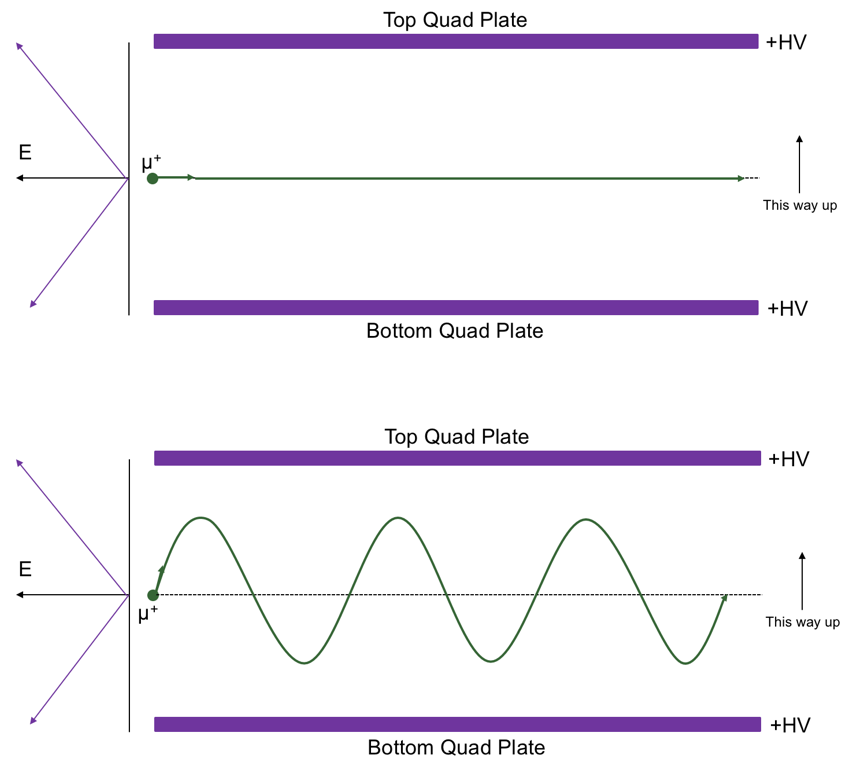
\includegraphics[scale=0.5]{Figures/vertoscillationdiagram.png}
\decoRule
\caption{Simplistic diagram of vertical betatron oscillations. If the muons were injected into the ring at y=0 and with no vertical momentum then the muon would stay perfectly horizontal as it travels through the ring until it decayed as shown in the top diagram. However the muons are not injected perfectly and so will posses a non-zero vertical momentum. The muons will then oscillate due to the restoring force from the quadrupole electric field, with the amplitude of the oscillation dependant on the initial direction as shown in the bottom diagram.}
\label{fig:vertoscillationdiagram.png}
\end{figure}

The pitch correction is so called because during vertical betatron oscillations, the pitch angle $\psi$, defined to be the angle between the momentum and the horizontal axis, varies harmonically with $\psi = \psi_{0}\mathrm{cos}\omega_{y}t$, where $\omega_{y}$ is the vertical betatron frequency $\omega_{y} = 2\pi{f_{y}}$ with $\omega_{y} = 2\pi\sqrt{n}f_{c} \simeq2\pi\times2.5$ MHz. This is illustrated in figure 7.6.

\begin{figure}[th]
\centering
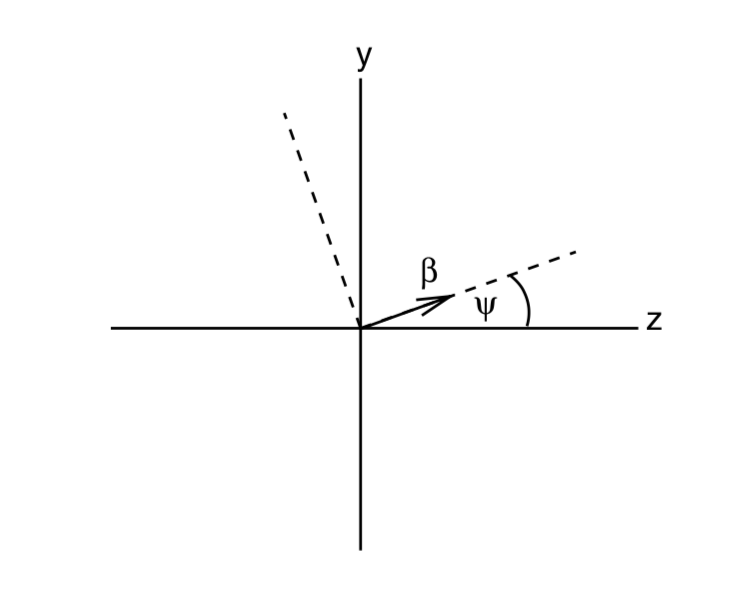
\includegraphics[scale=0.5]{Figures/pitcheffect.png}
\decoRule
\caption{A diagram showing the coordinate system of the pitching motion, $y$ = vertical direction, $z$ = azimuthal beam direction.}
\label{fig:pitcheffect.png}
\end{figure}

Using the assumption that the muons are all circulating on the magic radius, then $a_{\mu} - 1/(\gamma^{2}-1)=0 $ giving

\begin{equation}
\vec{\omega'_{a}}=-\frac{q}{m}[a_{\mu}\vec{B}-a_{\mu}\Big(\frac{\gamma}{\gamma+1}\Big)(\vec{\beta}\cdot\vec{B})\vec{\beta}]
\end{equation}

\noindent
Using $\vec{\omega_{a}}=-(q/m)a_{\mu}\vec{B}$. 

The coordinate system used in Figure 7.6 has y as the vertical axis, the z axis is the direction of propagation and $\vec{\beta}$ lying in the zy-plane. Using the assumptions

\begin{equation}
\vec{B}=\hat{y}B_{y}, \vec{\beta}=\hat{z}\beta_{z}+\hat{y}\beta_{y}=\hat{z}\bet {cos} \psi+\hat{y}\beta {sin} \psi, 
\end{equation}

\noindent
the equation below is derived.

\begin{equation}
\vec{\omega'_{a}} = - \frac{q}{m}[a_{\mu}\hat{y}B_{y}-a_{\mu}(\frac{\gamma}{\gamma + 1})\beta_{y}B_{y}(\hat{z}\beta_{z}+\hat{y}\beta_{y})].
\end{equation}

\noindent
Using the small angle approximation cos$\psi \simeq 1$ and sin$\psi \simeq \psi$ gives the following equations

\begin{equation}
\vec{\omega'_{ay}}=\omega_{a}[1-(\frac{\gamma}{\gamma + 1})\psi^2]
\end{equation}
\noindent
and
\begin{equation}
\vec{\omega'_{az}}=-\omega_{a}(\frac{\gamma - 1}{\gamma})\psi
\end{equation}

Instead $\vec{\omega'_{a}}$ can be resolved into components along the coordinate system $\vec{\beta}$ by use of the standard rotation formula. The equation for the transverse component of $\omega'$ is 
\begin{equation}
\omega_{\perp}=\vec{\omega'_{ay}}cos{\psi}-\vec{\omega'_{az}}{sin}\psi
\end{equation}

\noindent
Then use the small angle expansion cos$\psi \simeq 1 - \psi^{2}/2$ gives

\begin{equation}
\omega_{\perp} \simeq [1 - \frac{\psi^2}{2}]
\end{equation}

The vertical betatron oscillation frequency $f_{y}$ is approximately ten times faster than the g-2 oscillation frequency $f_{a}$. As vertical betatron oscillates ten times per g-2 oscillation, its effect on $\vec{\omega'_{a}}$ is averaged out, leading to $\vec{\omega'_{a}} \simeq \omega_{\perp}$ \cite{Reference1}. This gives

\begin{equation}
\omega_{a}\simeq \frac{q}{m}a_{\mu}B_{y}(1 - \frac{\psi^2}{2}) = - \frac{q}{m}a_{\mu}B_{y}(1 - \frac{\psi^{2}_{0}cos^{2}\omega_{y}t}{2})
\end{equation}

\noindent
Taking the time average of the oscillation yields the pitch correction $C_{p}$ and using the equation $<\psi^{2}_{0}> = n<y^{2}>/R^{2}_{0}$ gives the pitch correction 

\begin{equation}
C_{p} = - \frac{<\psi^2>}{2} = - \frac{<\psi^{2}_{0}>}{4} = - \frac{n}{4}\frac{<y^{2}>}{R^{2}_0}
\end{equation}

The vertical oscillations reduce the magnitude of $\omega_{a}$ and so the correction needs to be added to increase the value. In the 2001 BNL data set, the pitch correction was +0.27 $\pm$ 0.04 ppm \cite{Reference13}.

Before looking at the oscillations the average vertical position and vertical width were studied to characterise the overall behavior of the vertical components of the beam throughout the fill. These are shown in figures 7.7 and 7.8. It can be seen that up to 30$\mu{s}$ the beam is narrowing due to scraping as expected. After 30$\mu{s}$ however both distributions should be flat and this is not observed in either distribution. This decrease in the vertical width should only have a tiny effect on the pitch correction calculated. To check this the calculation of two pitch corrections was done using the vertical width distribution in Figure 7.8 at station 12. One at an early time of 30 $\mu{s}$ with a vertical width of 13.05 mm and a late time of 300 $\mu{s}$ which gave a vertical width value of 12.70 mm. A $C_p$ = 182 ppb was calculated at 30 $\mu{s}$ and  $C_p$ = 172 ppb at 300 $\mu{s}$. Therefore the unexpected varying of the vertical width only leads to a 10 ppb effect on the pitch correction, which is within the specifications. However the effect of the change in the beam position and width throughout the fill on the $\omega_{a}$ fits needs to be taken into account.

\begin{figure}[!h]
\centering 
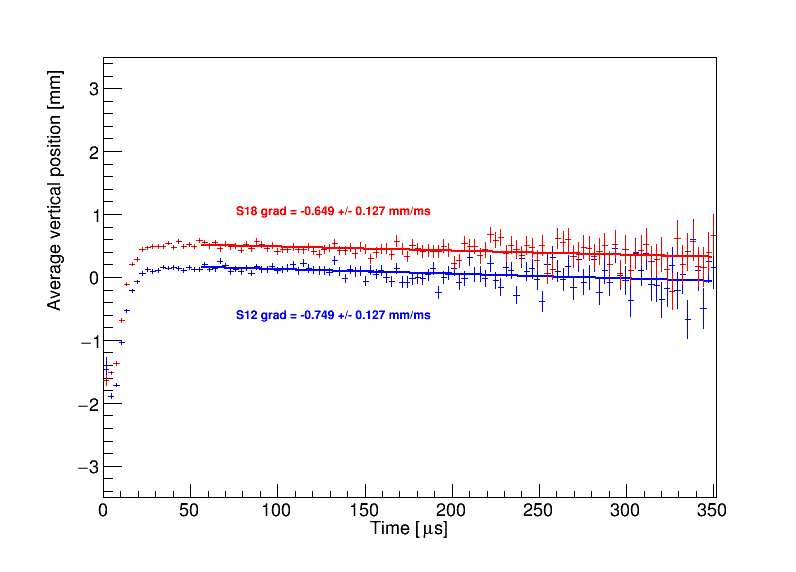
\includegraphics[scale=0.5]{Figures/AverageVerticalPosition_rebinMeanPeriod_both.png}
\decoRule
\caption{A plot showing the average vertical position of beam for both tracking stations (station 12 in blue and station 18 in red) showing an unexpected decrease throughout the fill.}
\label{fig:AverageVerticalPosition_rebinMeanPeriod_both.png}
\end{figure}

\begin{figure}[!h]
\centering 
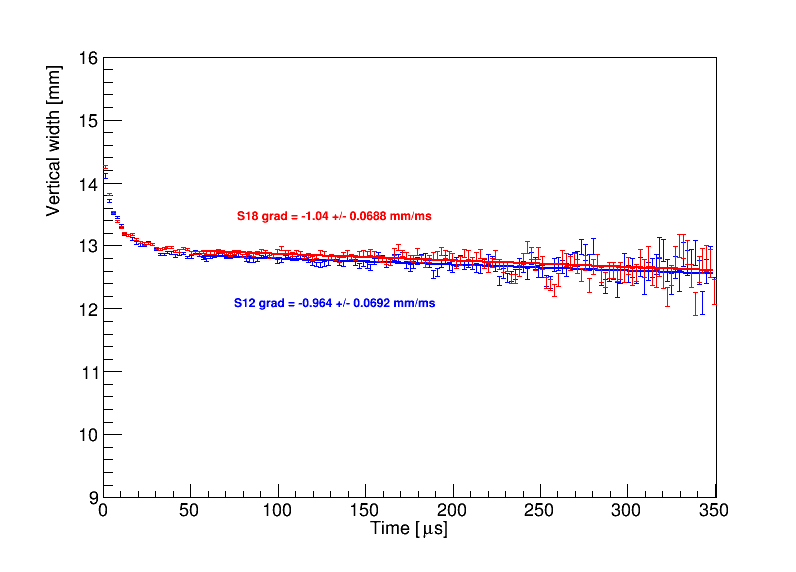
\includegraphics[scale=0.5]{Figures/AverageVerticalPosition_rebinWidthPeriod_both.png}
\decoRule
\caption{A plot showing the vertical width position of beam for both tracking stations (station 12 in blue and station 18 in red) showing an unexpected decrease throughout the fill.}
\label{fig:AverageVerticalPosition_rebinWidthPeriod_both.png}
\end{figure}

\section{Vertical betatron oscillations}

Before the observed change in mean and width during the fill the vertical beam frequencies were expected to be constant, but one explanation for them changing was that the quadrupole voltage was changing in an unexpected way during the fill. This would lead to the betatron frequencies also changing. To investigate this the extrapolated vertical position as a function of time from the trackers was used. The frequencies expected have a period of $\sim{450}$ ns, therefore the binning chosen was 10 ns. The average vertical position within each time bin is plotted versus the time in the fill. A fit is then applied, using a constant frequency as shown in Figures 7.9 and 7.10. An oscillation can clearly be seen in early times, at later times there is beam decoherence due to the momentum spread of the beam distribution. The $\chi^2$ from the fits is unacceptably large, and by looking at the fits at different times throughout the fill a change in frequency can be observed. Previously there had been evidence that there was a varying frequency in the radial beam oscillations and the fact that there was also evidence for this in the vertical beam oscillations indicated that the quadrupole field was indeed varying throughout the fill. This variation needed to be characterised more precisely so that it could be included in the $\omega_{a}$ fit function, and not distort the extracted value of $\omega_{a}$.

\begin{figure}[!h]
\centering 
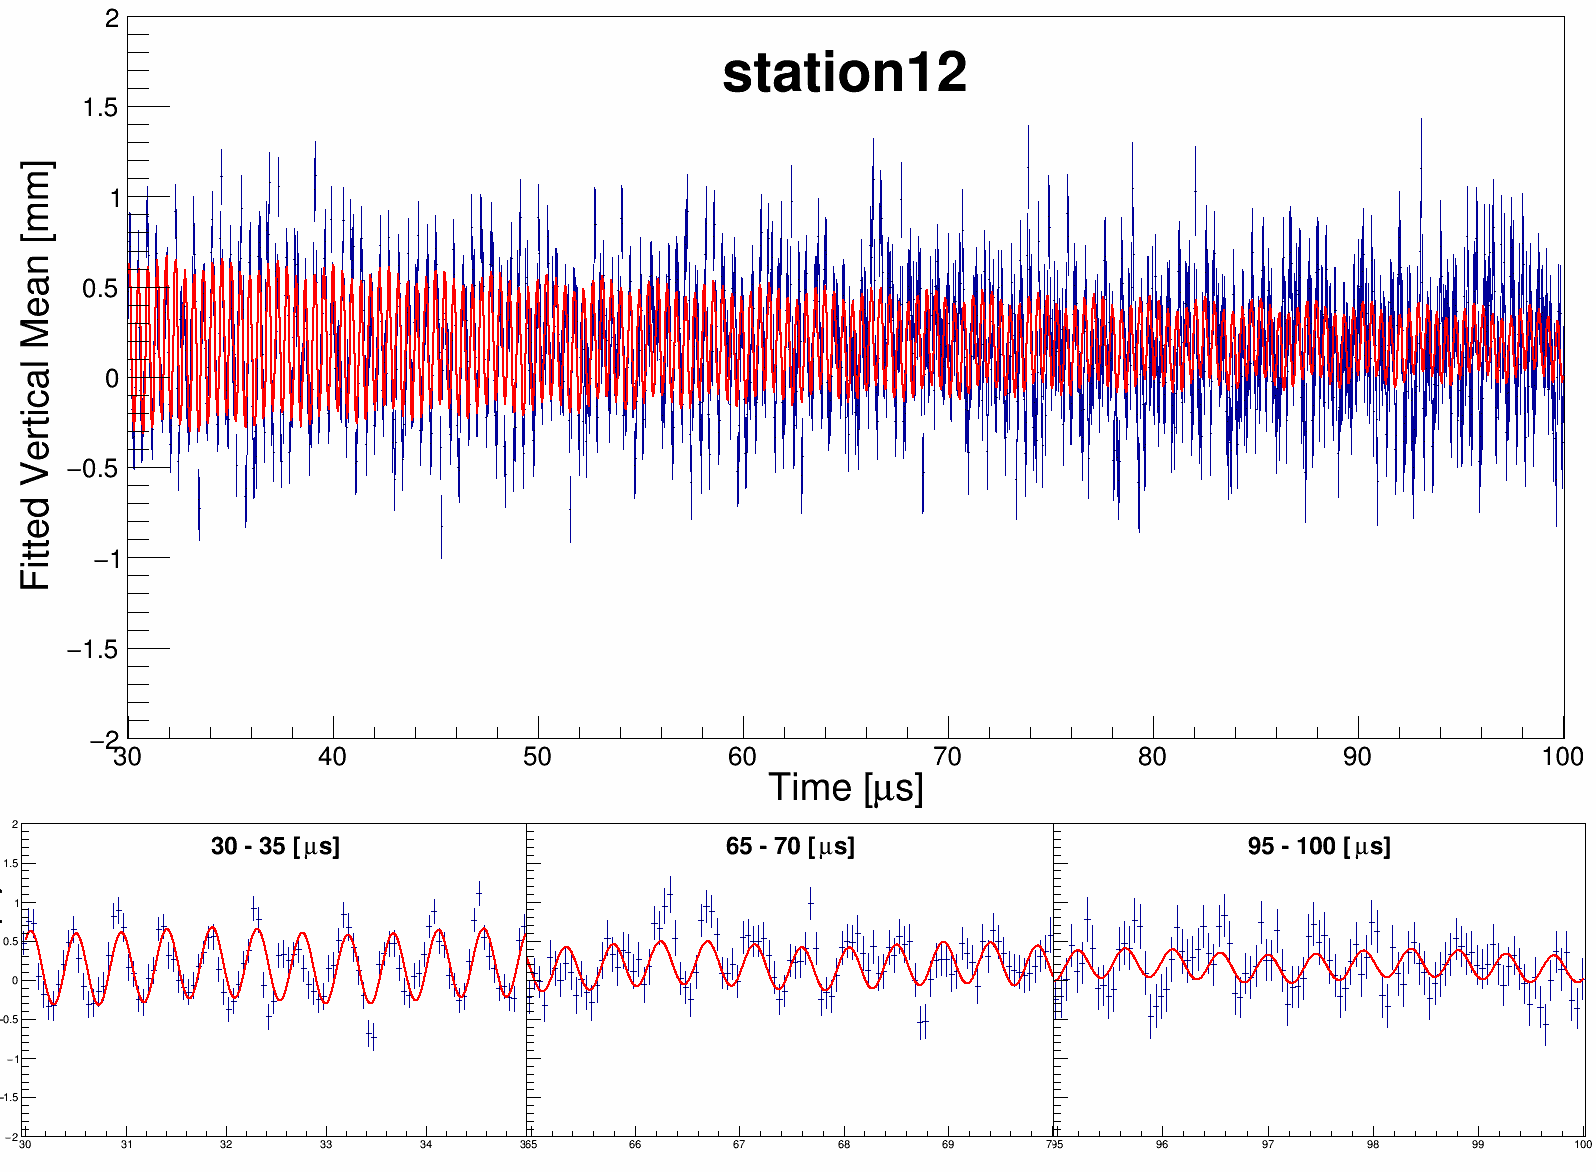
\includegraphics[scale=0.25]{Figures/AverageVerticalPosition_exponentialFit_station12.png}
\decoRule
\caption{A plot of the average vertical position throughout the fill measured at station 12. It shows that at early times oscillations are clearly visible and can be fitted well. The fit becomes worse a later times as the oscillations become less clearly visible.}
\label{fig:AverageVerticalPosition_exponentialFit_station12.png}
\end{figure}

\begin{figure}[!h]
\centering 
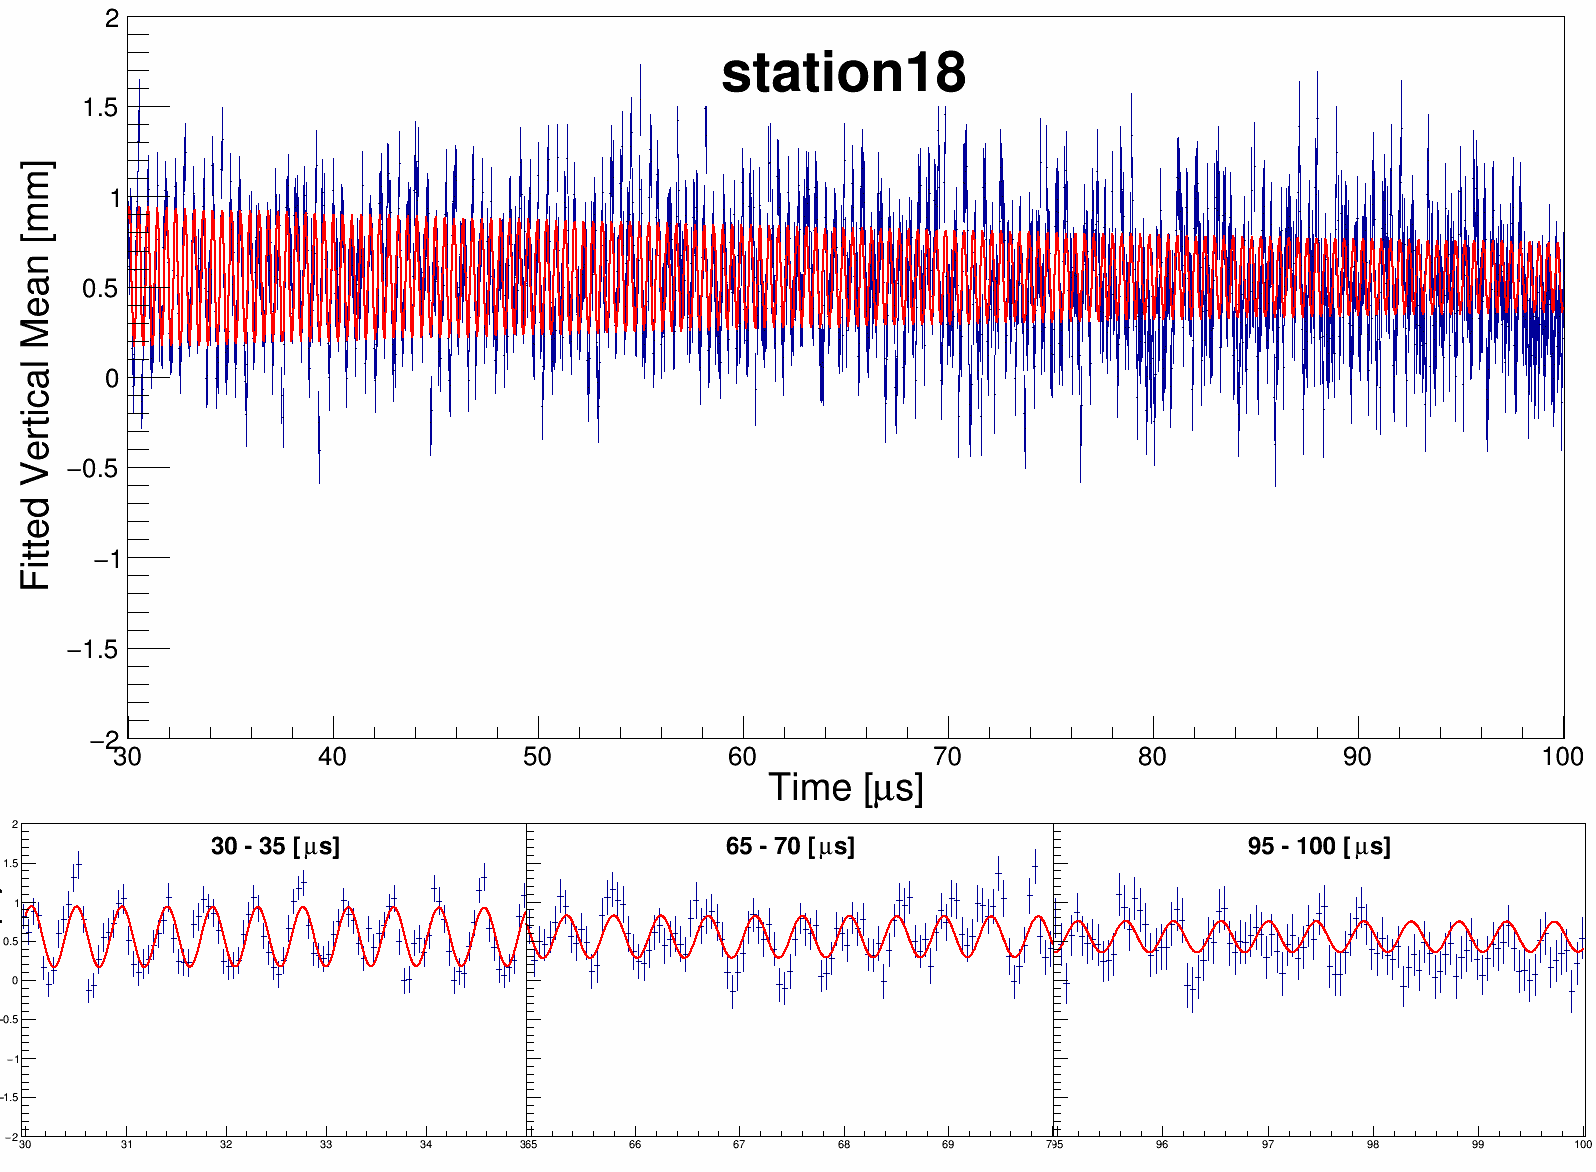
\includegraphics[scale=0.25]{Figures/AverageVerticalPosition_exponentialFit_station18.png}
\decoRule
\caption{A plot of the average vertical position throughout the fill measured at station 18. It shows that at early times oscillations are clearly visible and can be fitted well. The fit becomes worse a later times as the oscillations become less clearly visible.}
\label{fig:AverageVerticalPosition_exponentialFit_station18.png}
\end{figure}

\section{Varying beam oscillation frequencies}

As mentioned previously, the oscillation of the radial mean has a longer period and therefore is easier to measure with limited statistics. The variation in the radial frequency can be converted into an expected variation vertically using equation 7.24. However the equations are for ideal conditions (complete quadrupole coverage), so it is crucial to measure the vertical frequency variation independently. To investigate this variation in frequency further, time slices from the average vertical position were then taken and a Gaussian fit in the range $\pm$ 35 mm was performed to each time slice to obtain the vertical mean and vertical width. It can be seen from the plots in figure 7.11 that the width as well as the mean is varying throughout the fill. Figure 7.12 and figure 7.13 show the results of the fit in a 10 $\mu$s time slice from 20-25$\mu$s for the vertical width and vertical mean for station 12 and station 18 respectively. Looking at these distributions it can be seen that there are multiple frequencies in both. The individual frequencies that are in the distributions can be determined by doing an Fast Fourier Transform (FFT) on the vertical width and vertical mean. Figures 7.14 and 7.15 show the FFT for the fitted vertical mean (in blue) and the vertical width (in red) with the individual frequencies labelled for station 12 and station 18. However an FFT is not the most accurate method for obtaining the frequency values, particularly when looking for variations in frequency. Therefore fits were applied to the distributions to obtain more accurate frequency values, using the main frequencies from the FFT results as the initial guesses for the fit. Here 3 iterations of fits were carried out. The distributions were then split up into 10 $\mu$s sections 
% were they split up before or after you applied the fits to get the accurate frequency values? 
as we have limited statistics and fitted separately to look for variation/trends throughout the fill. Figures 7.16 - 7.23 show the fits for the vertical mean and vertical width for both stations at an early and late time. 

\begin{figure}[!h]
\centering 
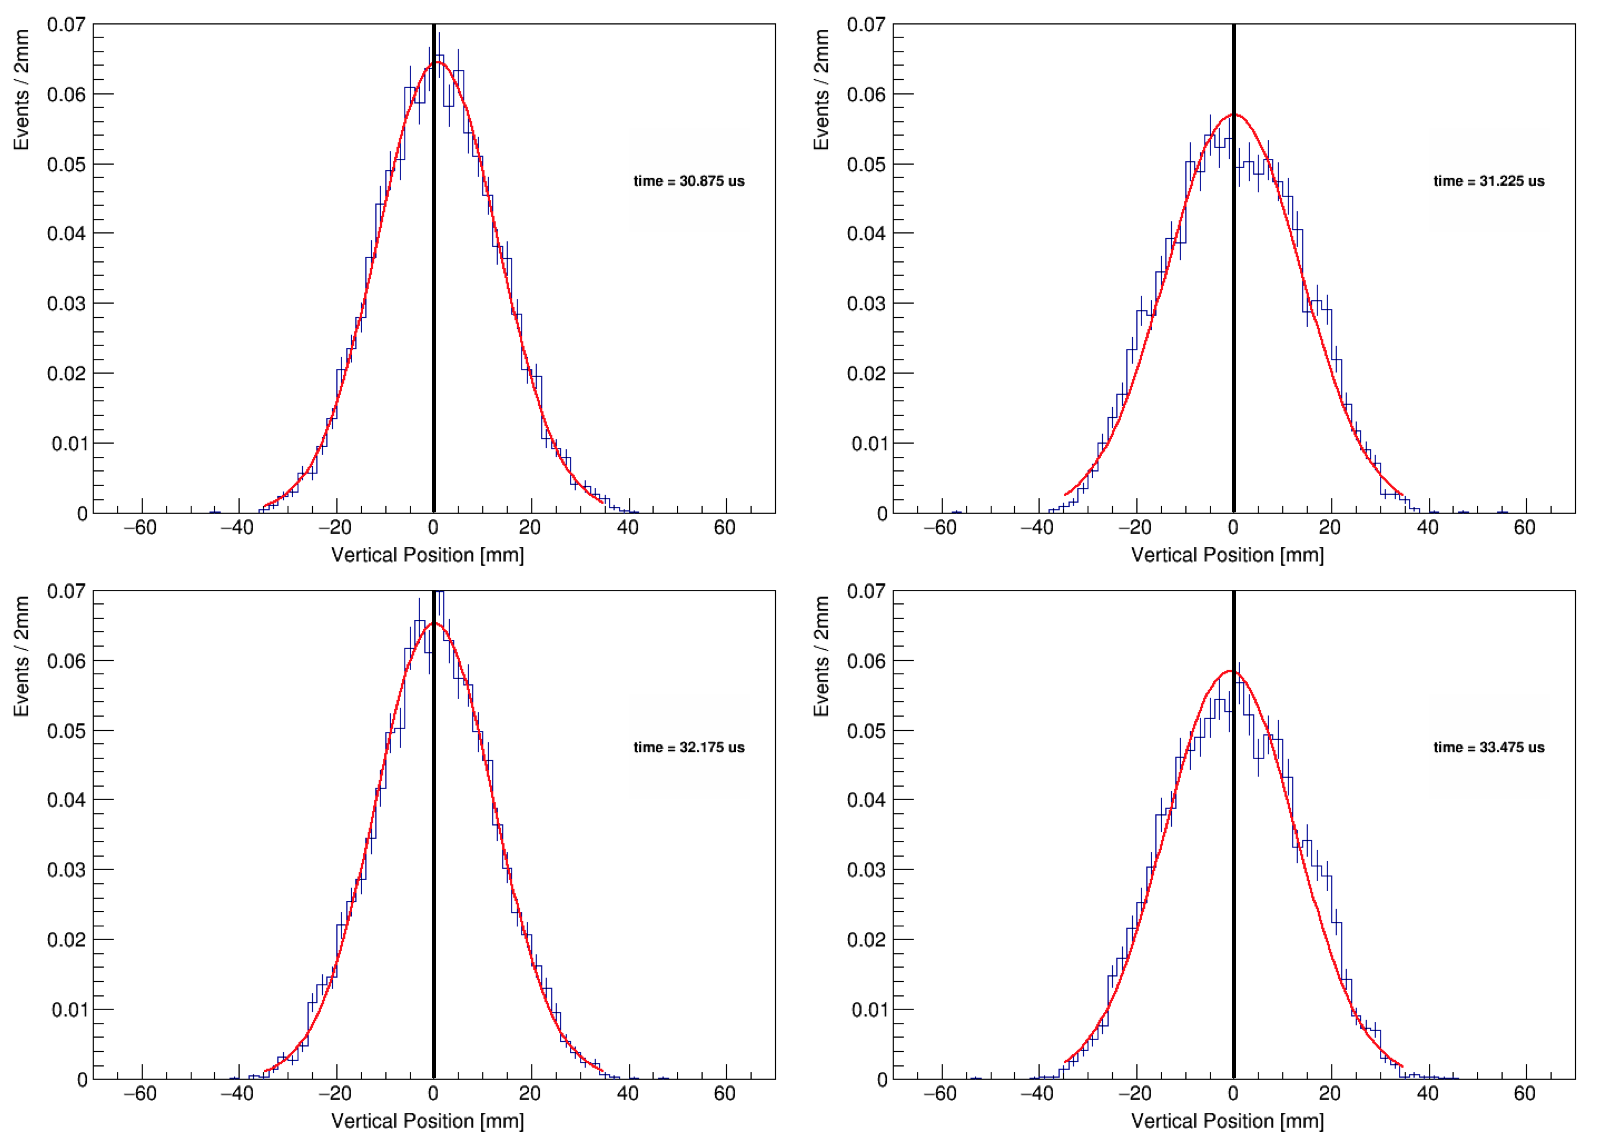
\includegraphics[scale=0.5]{Figures/verticalpositions.png}
\decoRule
\caption{Plots showing how the vertical positions mean and width vary with time.}
\label{fig:verticalpositions.png}
\end{figure}

\begin{figure}[!h]
\centering 
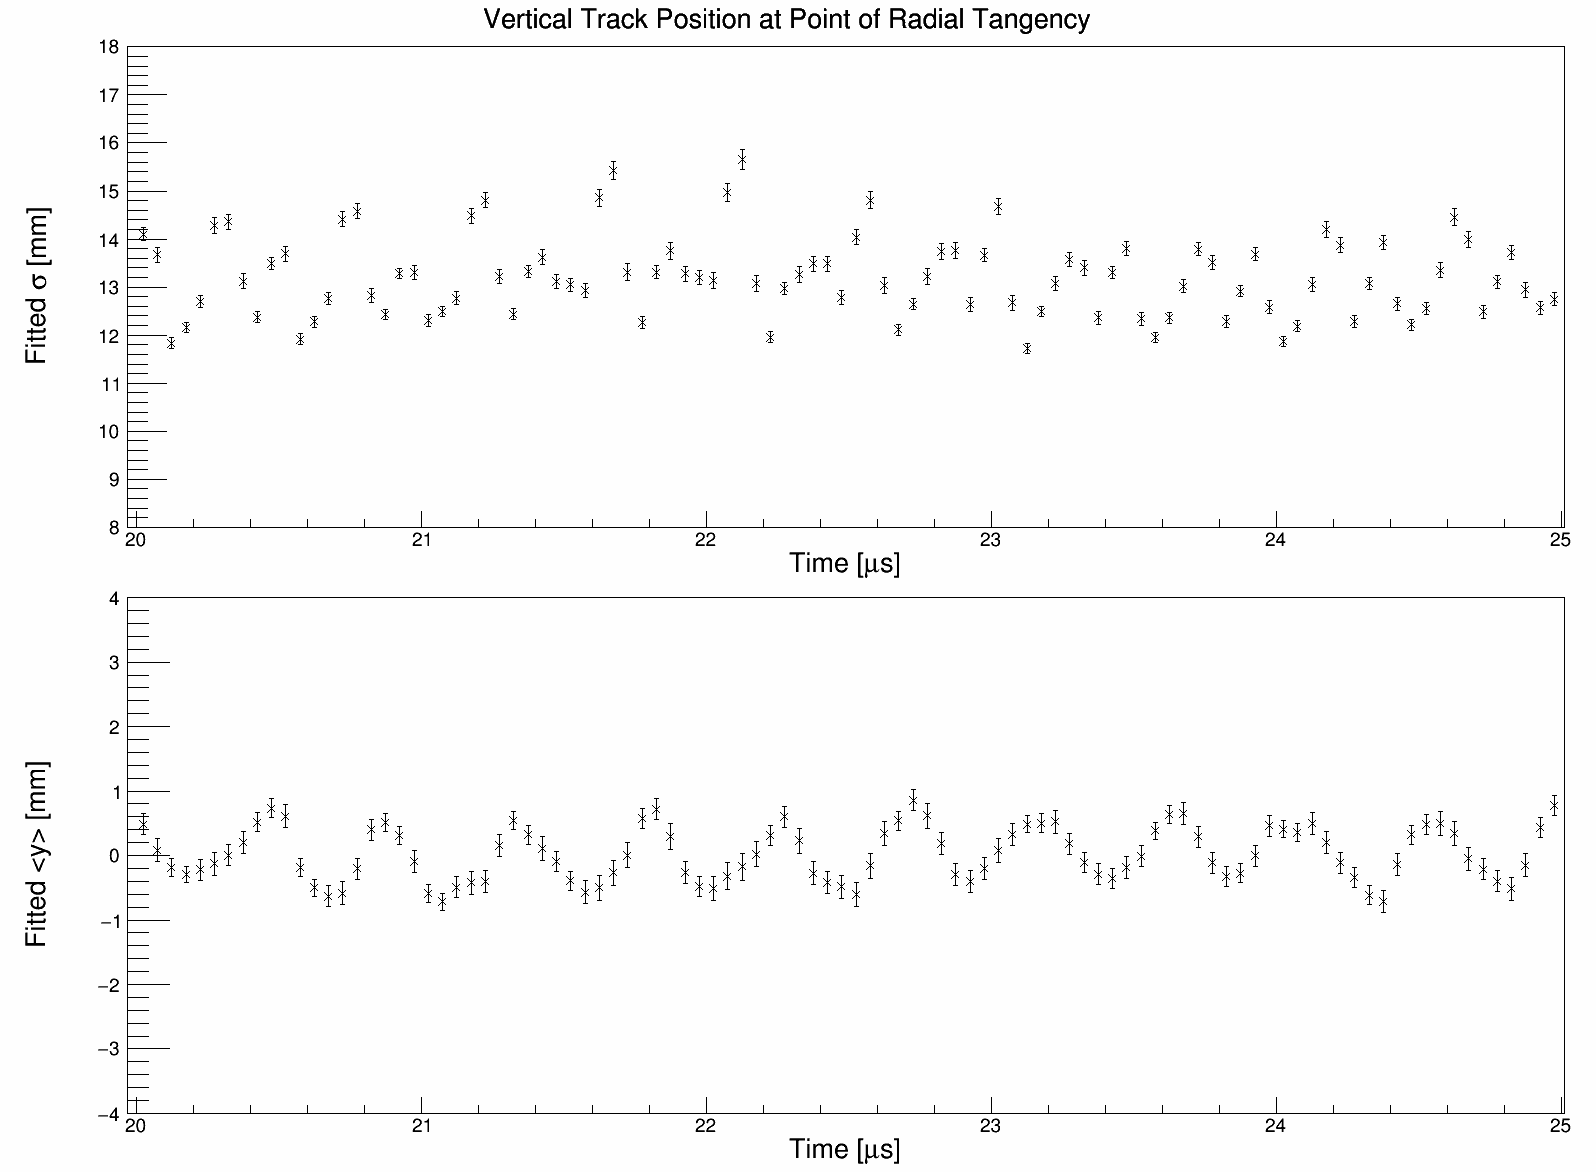
\includegraphics[scale=0.2]{Figures/Width_mean_comparison_station12.png}
\decoRule
\caption{Comparison of the mean and width distributions for station 12 at early times 30-40$\mu$s, display that a mixture of frequencies are included in the distribution.}
\label{fig:Width_mean_comparison_station12}
\end{figure}

\begin{figure}[!h]
\centering 
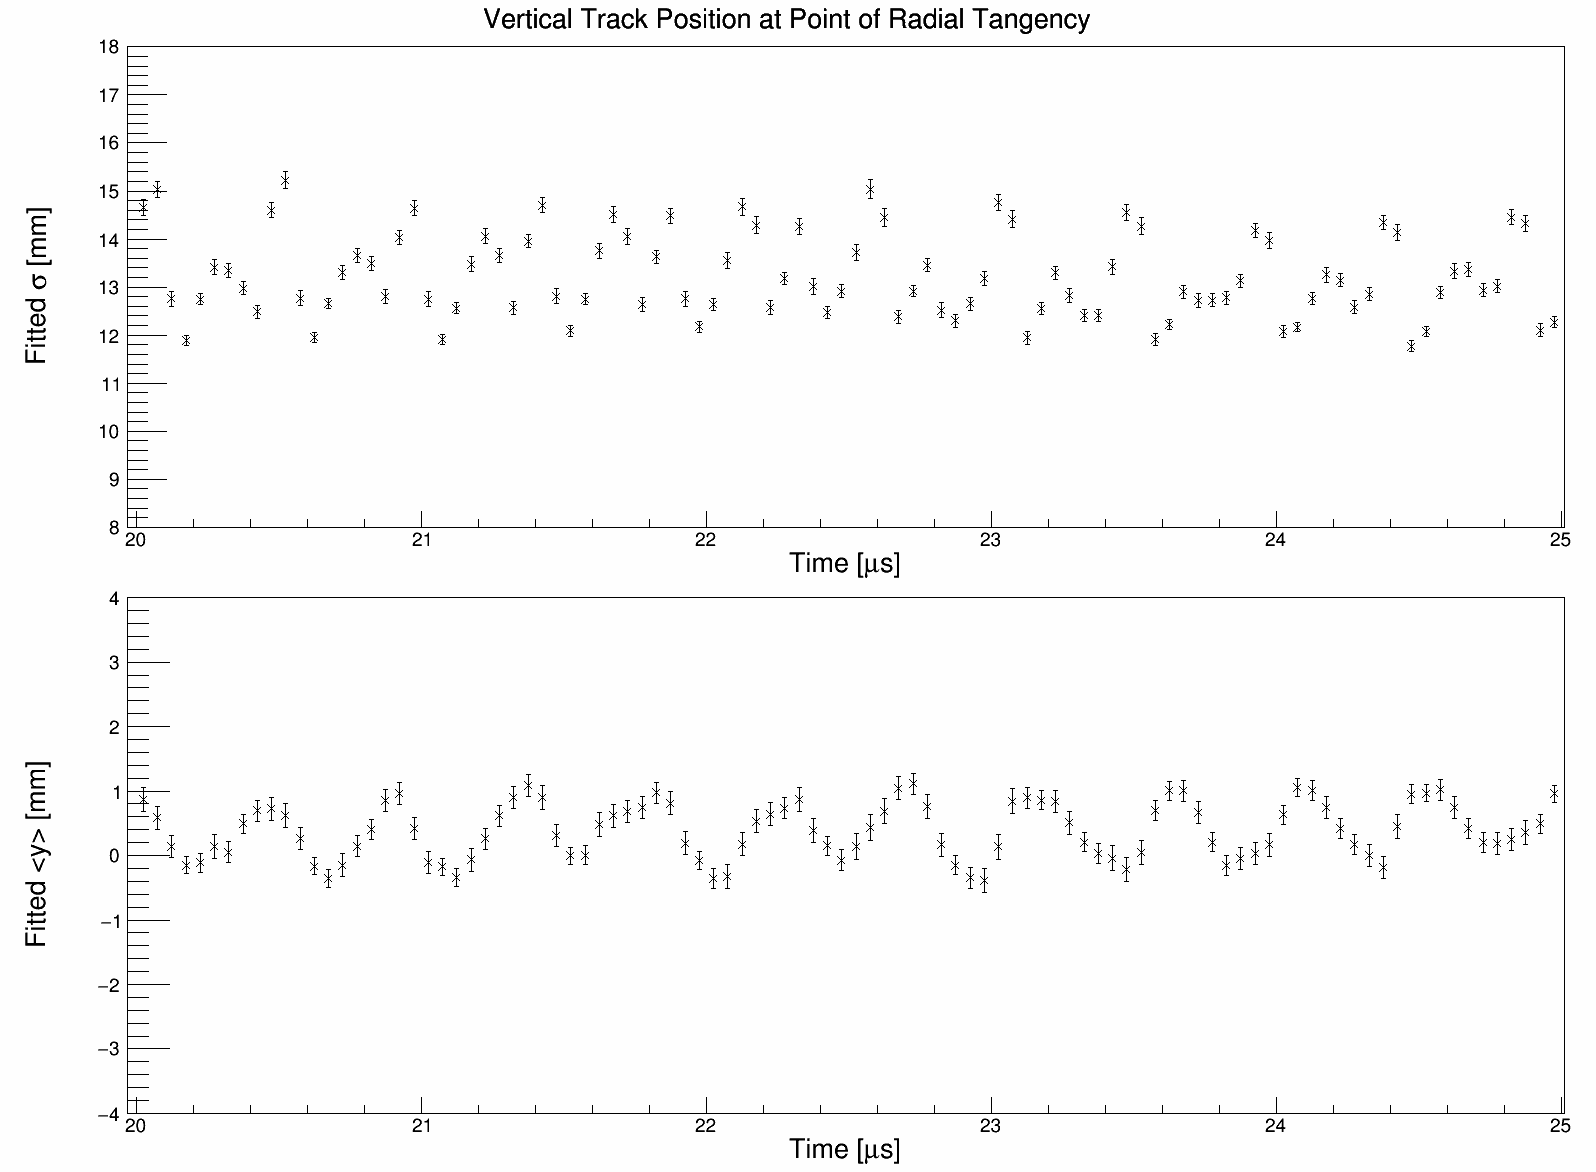
\includegraphics[scale=0.2]{Figures/Width_mean_comparison_station18.png}
\decoRule
\caption{Comparison of the mean and width distributions for station 18 at early times 30-40$\mu$s, display that a mixture of frequencies are included in the distribution.}
\label{fig:Width_mean_comparison_station18}
\end{figure}

\begin{figure}[!h]
\centering 
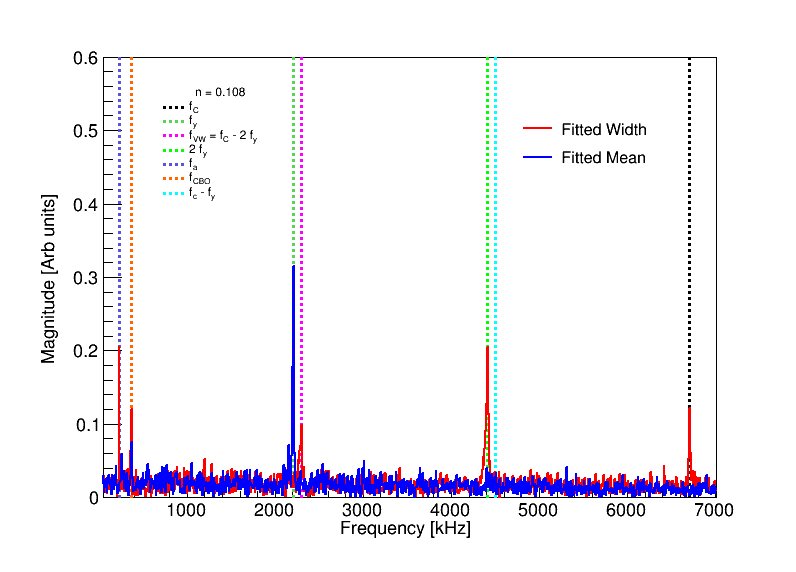
\includegraphics[scale=0.5]{Figures/FFT_fittedWidth_fittedMean_station12.png}
\decoRule
\caption{FFT at station 12 using the 60 hour dataset}
\label{fig:FFT_fittedWidth_fittedMean_station12.png}
\end{figure}

\begin{figure}[!h]
\centering 
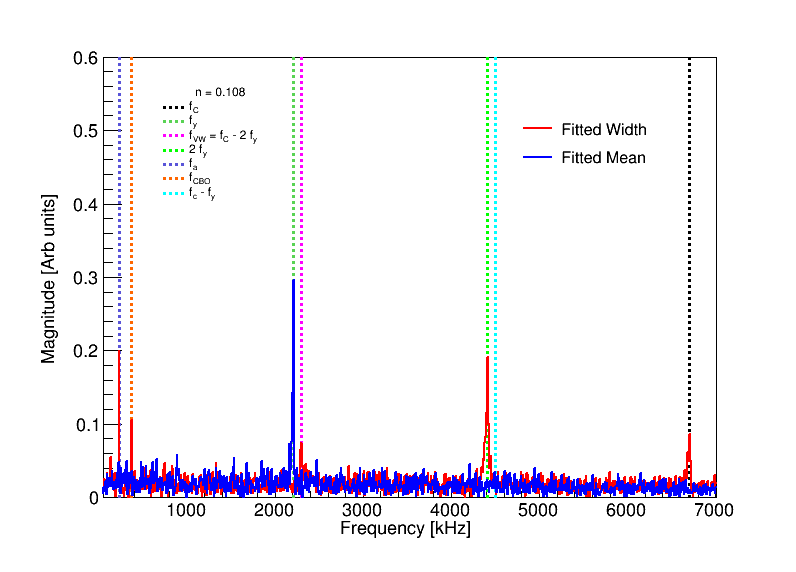
\includegraphics[scale=0.5]{Figures/FFT_fittedWidth_fittedMean_station18.png}
\decoRule
\caption{FFT at station 18 using the 60 hour dataset}
\label{fig:FFT_fittedWidth_fittedMean_station18.png}
\end{figure}

\begin{figure}
\centering
\begin{minipage}{.5\textwidth}
  \centering
  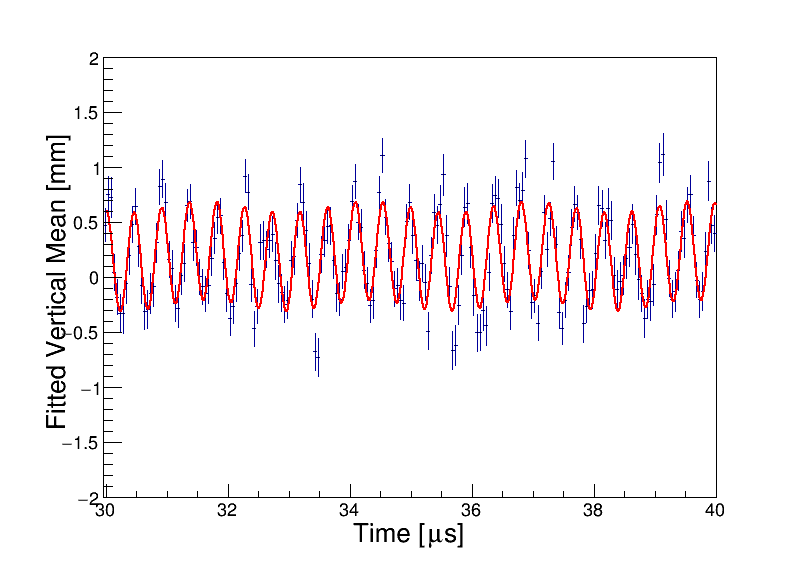
\includegraphics[width=\linewidth]{Figures/Mean_30_40_s12.png}
  \captionof{figure}{A plot of the fitted vertical mean in a 10 $\mu$s slice between 30 $\mu$s and 40 $\mu$s measured at station 12.}
  \label{fig:Mean_30_40_s12.png}
\end{minipage}%
\begin{minipage}{.5\textwidth}
  \centering
  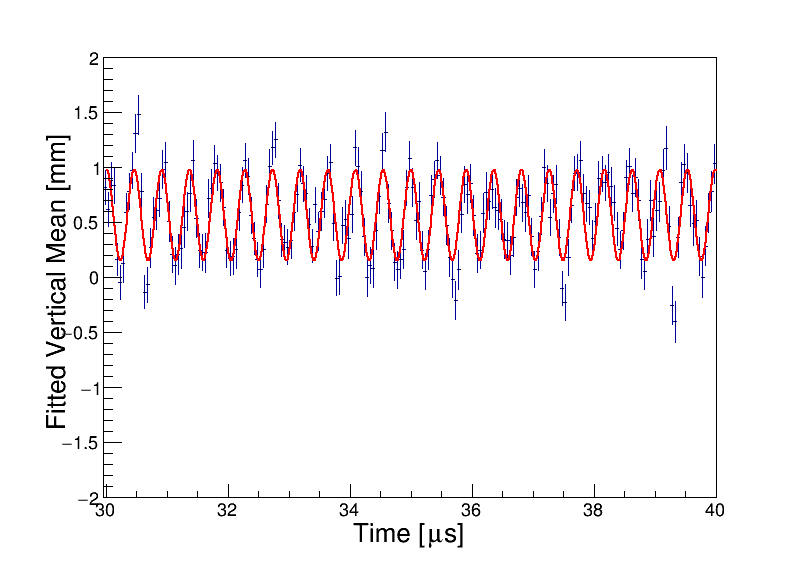
\includegraphics[width=\linewidth]{Figures/Mean_30_40_s18.png}
  \captionof{figure}{A plot of the fitted vertical mean in a 10 $\mu$s slice between 30 $\mu$s and 40 $\mu$s measured at station 18.}
  \label{fig:Mean_30_40_s18.png}
\end{minipage}
\end{figure}

\begin{figure}
\centering
\begin{minipage}{.5\textwidth}
  \centering
  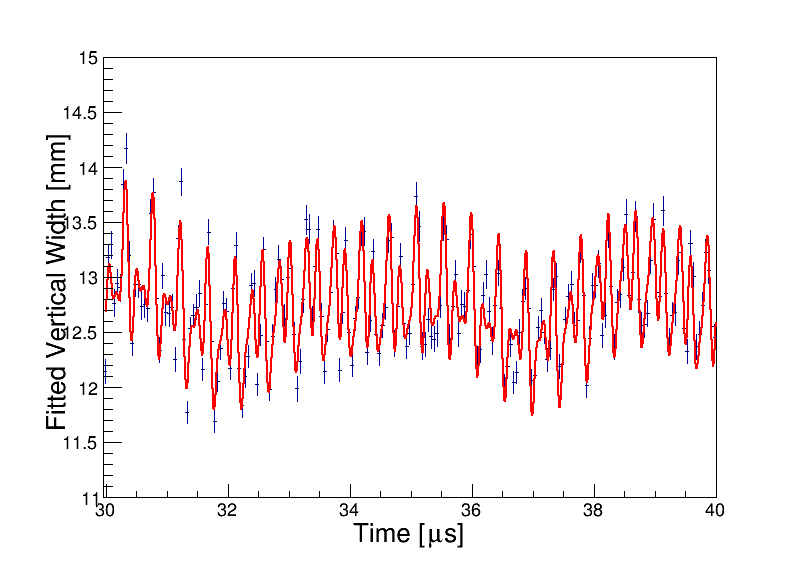
\includegraphics[width=\linewidth]{Figures/Width_30_40_s12.png}
  \captionof{figure}{A plot of the fitted vertical width in a 10 $\mu$s slice between 30 $\mu$s and 40 $\mu$s measured at station 12.}
  \label{fig:Width_30_40_s12.png}
\end{minipage}%
\begin{minipage}{.5\textwidth}
  \centering
  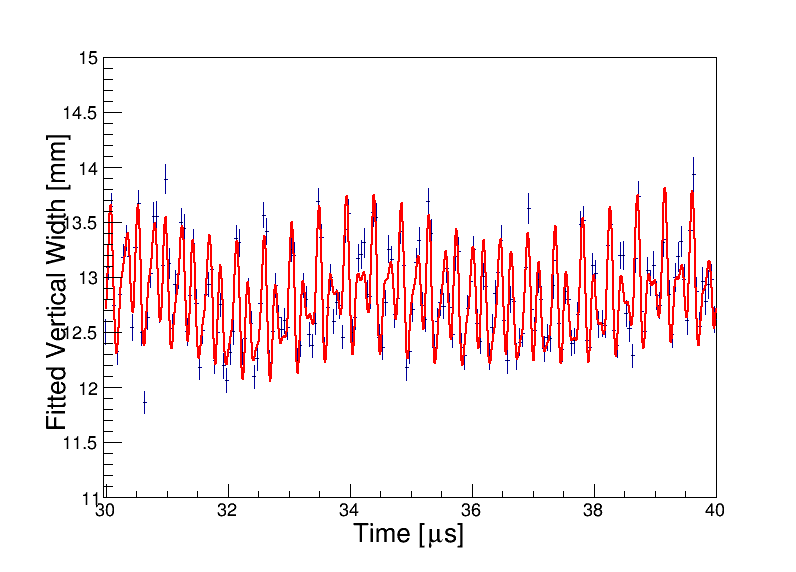
\includegraphics[width=\linewidth]{Figures/Width_30_40_s18.png}
  \captionof{figure}{A plot of the fitted vertical mean in a 10 $\mu$s slice between 30 $\mu$s and 40 $\mu$s measured at station 18.}
  \label{fig:Width_30_40_s18.png}
\end{minipage}
\end{figure}

%Do these next 4 (from 7.20 onwards) have a varying frequency?

\begin{figure}
\centering
\begin{minipage}{.5\textwidth}
  \centering
  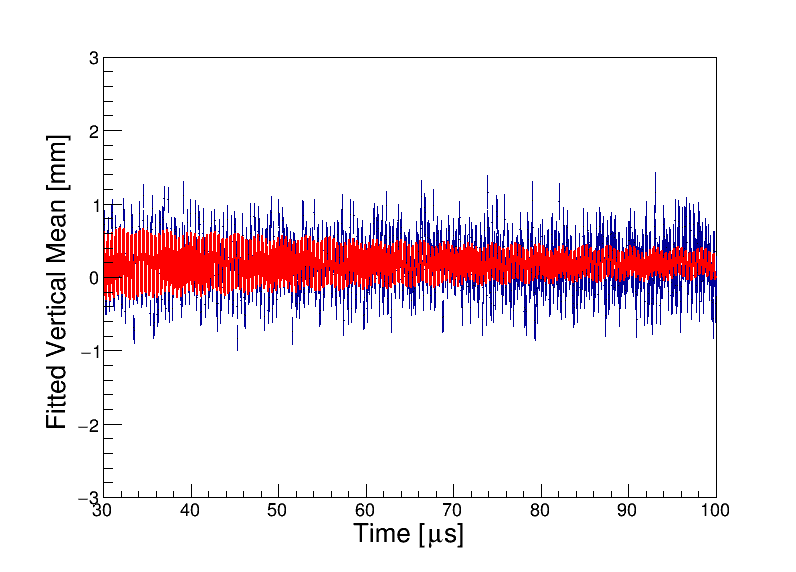
\includegraphics[width=\linewidth]{Figures/VertMeanTest_iterExp_station12.png}
  \captionof{figure}{A plot of the final fitted vertical mean in over 70 $\mu$s  between 30 $\mu$s and 100 $\mu$s measured at station 12.}
  \label{fig:VertMeanTest_iterExp_station12.png}
\end{minipage}%
\begin{minipage}{.5\textwidth}
  \centering
  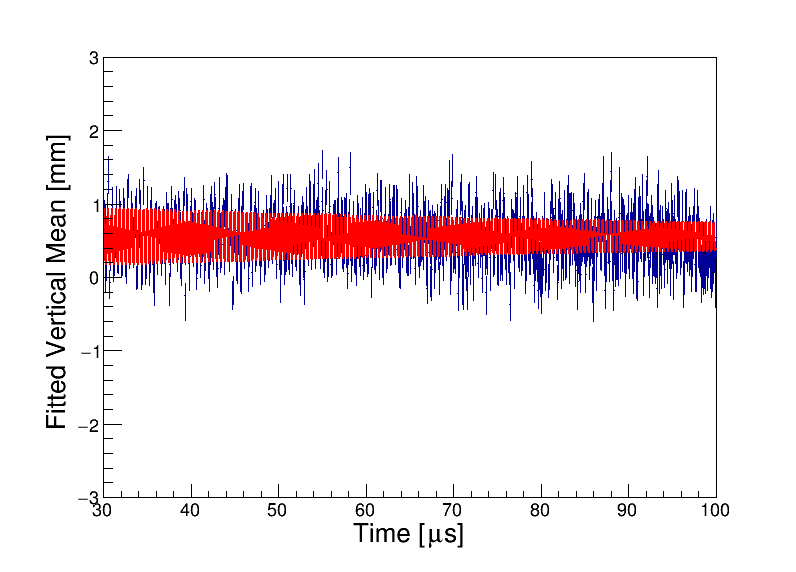
\includegraphics[width=\linewidth]{Figures/VertMeanTest_iterExp_station18.png}
  \captionof{figure}{A plot of the final fitted vertical mean in over 70 $\mu$s  between 30 $\mu$s and 100 $\mu$s measured at station 18.}
  \label{fig:VertMeanTest_iterExp_station18.png}
\end{minipage}
\end{figure}

\begin{figure}
\centering
\begin{minipage}{.5\textwidth}
  \centering
  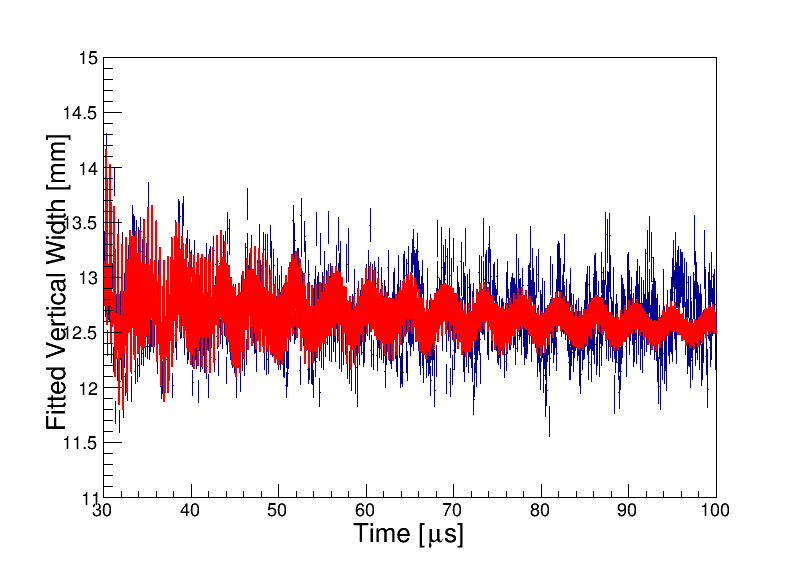
\includegraphics[width=\linewidth]{Figures/VertWidthTest_iterExp_station12.png}
  \captionof{figure}{A plot of the final fitted vertical width in over 70 $\mu$s  between 30 $\mu$s and 100 $\mu$s measured at station 12.}
  \label{fig:VertWidthTest_iterExp_station12.png}
\end{minipage}%
\begin{minipage}{.5\textwidth}
  \centering
  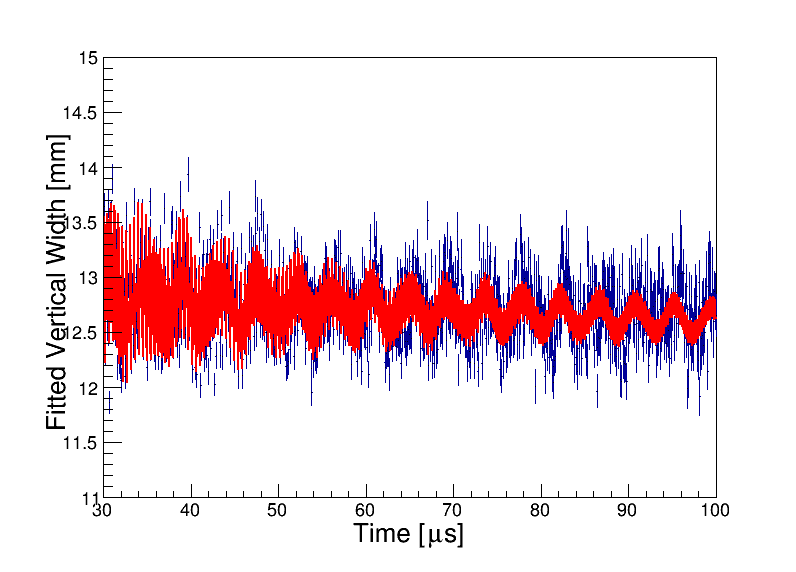
\includegraphics[width=\linewidth]{Figures/VertWidthTest_iterExp_station18.png}
  \captionof{figure}{A plot of the final fitted vertical width in over 70 $\mu$s  between 30 $\mu$s and 100 $\mu$s measured at station 18.}
  \label{fig:VertWidthTest_iterExp_station18.png}
\end{minipage}
\end{figure}

Here the 9 day dataset is used for these plots as the statistics are higher compared to 60 hour dataset. However the limited statistics mean that only the $f_{y}$ and $f_{VW}$ can be fitted.

Table 7.1 shows the difference in the frequencies observed in the FFTs calculated using the field index 0.108 and calculated using the fit with an exponentially decaying sinusoid for the time period 30-40$\mu$s.

\begin{table}[h!]
\begin{center}
 \begin{tabular}{||c | c | c | c | c | c||} 
 \hline
 Quantity & Expression & Frequency [MHz] & Period [\mu{s}] & Frequency [MHz] & Period [\mu{s}] \\ [0.5ex] 
 \hline\hline
 f_{a} & $\frac{e}{2\pi{mc}}a_{\mu}B$ & 0.229
 & 4.37 & 0.221 & 4.525\\ 
 \hline
 f_{c} & $\frac{\nu}{\pi{R_0}}$ & 6.700 & 0.149 & 6.700 & 0.149 \\
 \hline
 f_{y} & $\sqrt{n}f_{c}$ & 2.202 & 0.454 & 2.211 & 0.452 \\
 \hline
 f_{CBO} & f_{c} - f_{x} & 0.372 & 2.688 & 0.376 & 2.667\\ 
 \hline
 f_{VW} & f_{c} - 2f_{y} & 2.296 & 0.436 & 2.297 & 0.435\\ 
 \hline
\end{tabular}
\caption{Frequencies in the g-2 storage ring for the 60hr data with a field index of n=0.108, showing the frequencies determined for the FFT along with the frequencies calculated using the fits.}
\end{center}
\end{table}

\subsection{Comparison with radial frequency variation.}

The relationship between the vertical betatron oscillation frequency and the radial CBO frequency is shown below

\begin{equation}
f_{y} = f_{CBO}\sqrt{\frac{2f_{c}}{f_{CBO}}-1}
\end{equation}
This is derived from equations for continuous quads rather than the segmented quads of the experiment. 

\begin{figure}[!h]
\centering 
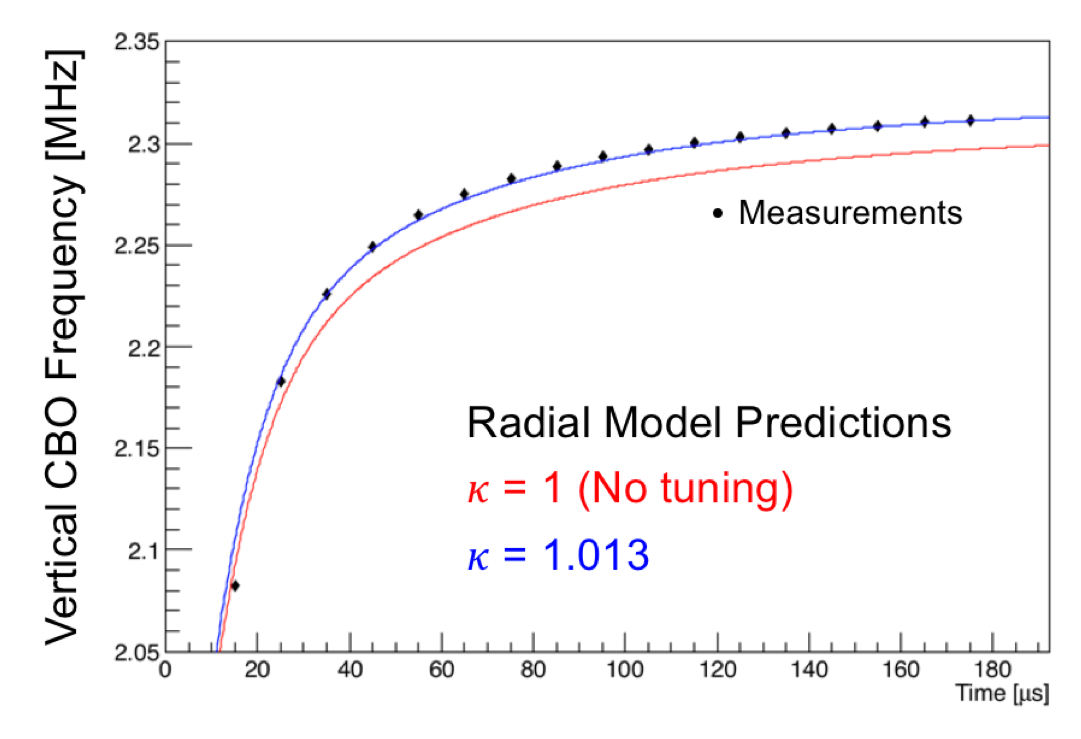
\includegraphics[scale=0.7]{Figures/VCBOvsFREQ.png}
\decoRule
\caption{Comparison of the vertical CBO oscillation calculated using the vertical betatron oscillation and the vertical CBO observed expermentally. A tune of 1.03 is required to create an agreement between the two values.}
\label{fig:VCBOvsFREQ}
\end{figure}

Figure 7.24 displays the observed vertical CBO frequency distribution obtained from the 10 $\mu$s fits to the tracker data. The measurements are the black dots, the red is from the equation using the frequency from the radial. In order to obtain a good agreement between the two, an additional multiplicative factor needed to be applied to $f_{y}$. This factor corresponds to a 1.3$\%$ increase, and is attributed to the equations being based on 100$\%$ quad coverage, which is not the case in the experiment. With this factor established, it is now possible to convert between the measured variation in frequency radially and vertically. This is important because the radial CBO, and its variation throughout the fill, can be fitted more precisely than the vertical frequencies. The impact of adding the variation of the vertical oscillations to the $\omega_{a}$ fits, including this parameter is discussed in the next section.  

\section{Fitting $\omega_{a}$}

\begin{figure}[!h]
\centering 
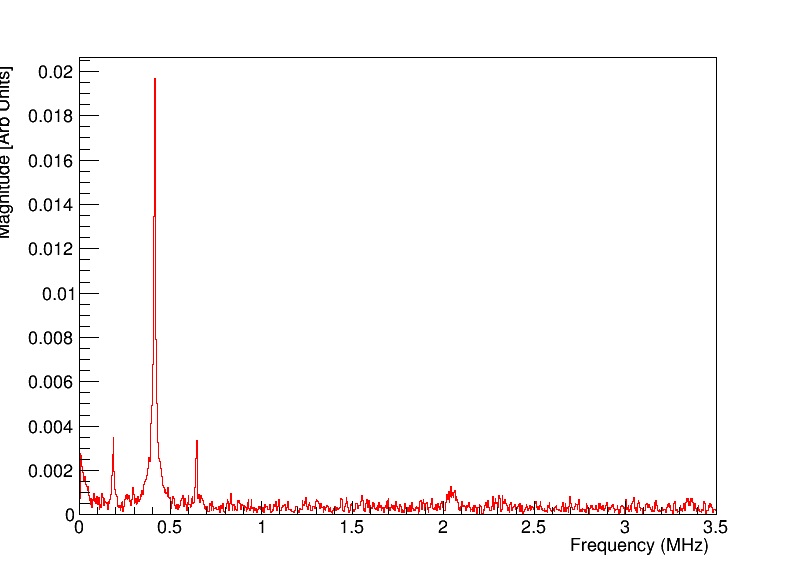
\includegraphics[scale=0.5]{Figures/5par_fft.png}
\decoRule
\caption{Plot of an FFT for the 5 parameter fit}
\label{fig:5par_fft}
\end{figure}

\iffalse
\begin{figure}[!h]
\centering 
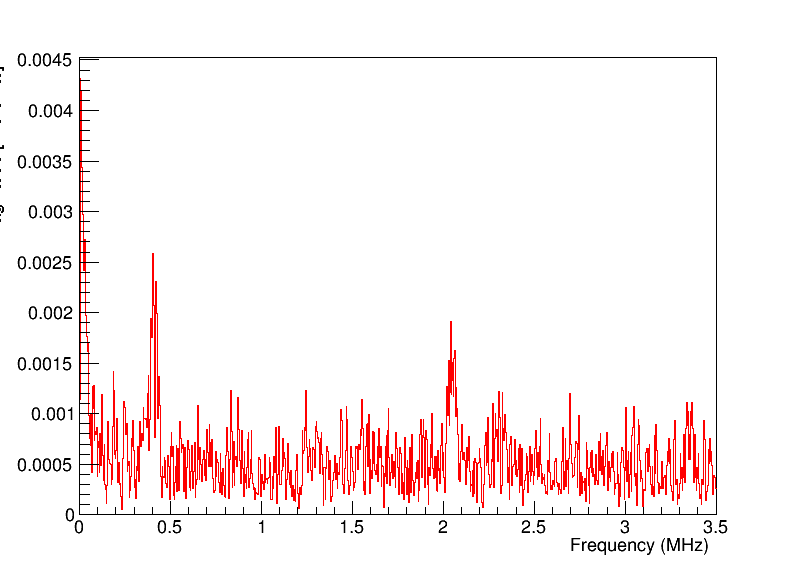
\includegraphics[scale=0.5]{Figures/9par_fft.png}
\decoRule
\caption{Plot of an FFT for the 9 parameter fit}
\label{fig:9par_fft}
\end{figure}

\begin{figure}[!h]
\centering 
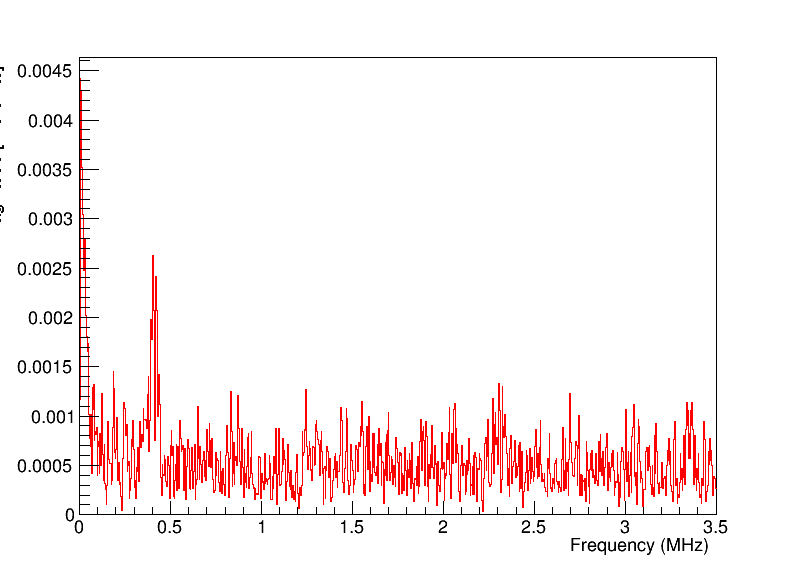
\includegraphics[scale=0.5]{Figures/verCBO_fft.png}
\decoRule
\caption{FFT for verCBO}
\label{fig:verCBO_fft}
\end{figure}

\begin{figure}[!h]
\centering 
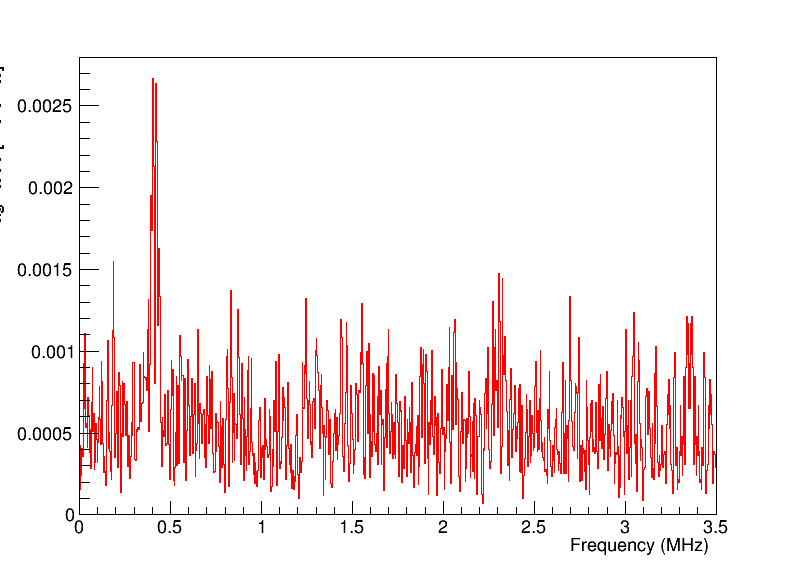
\includegraphics[scale=0.5]{Figures/vCBOML_fft.png}
\decoRule
\caption{FFT for vCBOML}
\label{fig:vCBOML_fft}
\end{figure}

\begin{figure}[!h]
\centering 
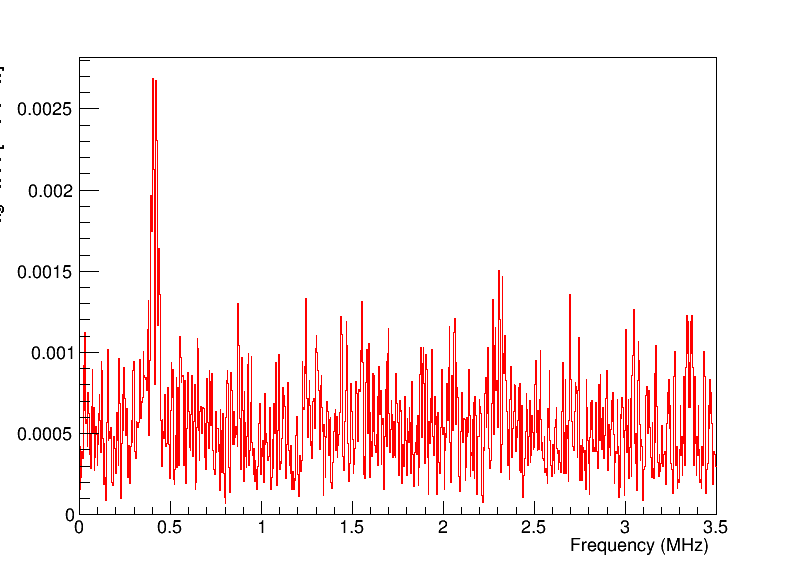
\includegraphics[scale=0.5]{Figures/fullCBOML_fft.png}
\decoRule
\caption{FFT for fullCBOML}
\label{fig:fullCBOML_fft}
\end{figure}
\fi

\begin{figure}[!h]
\centering 
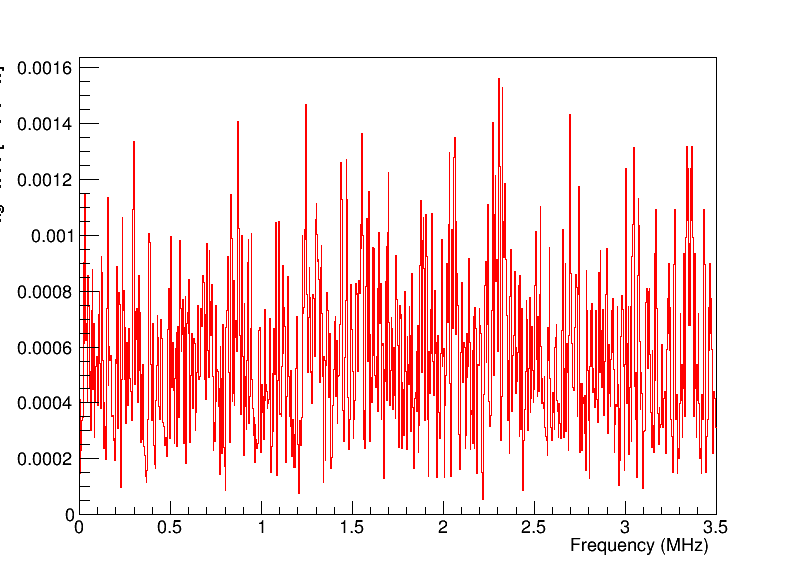
\includegraphics[scale=0.5]{Figures/varCBOnew_fft.png}
\decoRule
\caption{FFT for varCBOnew}
\label{fig:varCBOnew_fft}
\end{figure}

\begin{figure}[!h]
\centering 
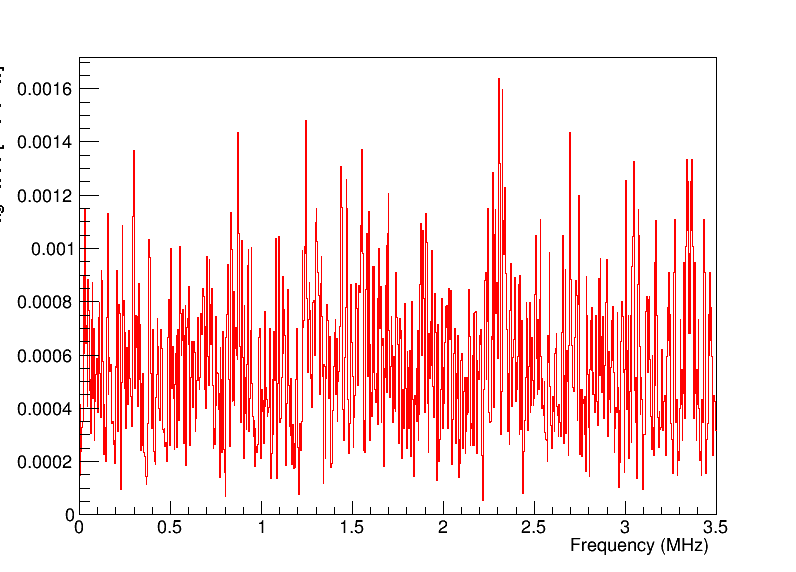
\includegraphics[scale=0.5]{Figures/varCBO9day_fft.png}
\decoRule
\caption{FFT for varCBO9day}
\label{fig:varCBO9day_fft}
\end{figure}

\iffalse
\begin{figure}[!h]
\centering 
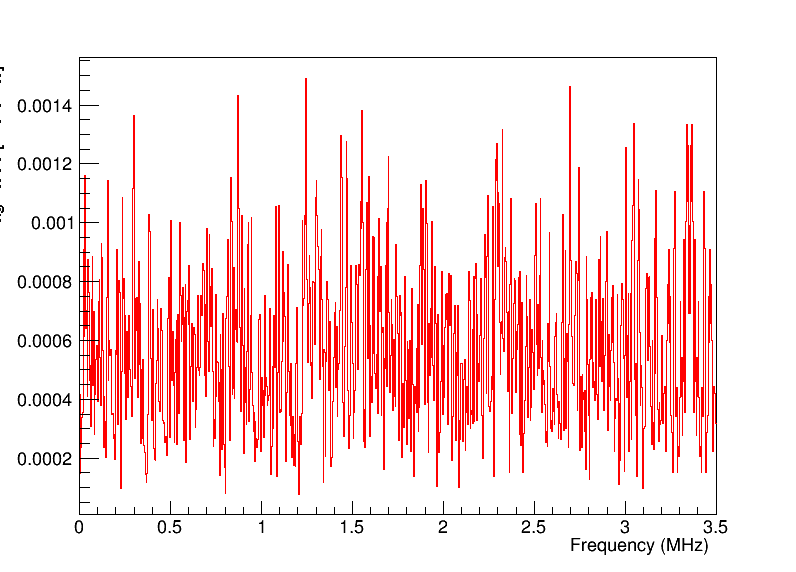
\includegraphics[scale=0.5]{Figures/varCBOelba_fft.png}
\decoRule
\caption{FFT for varCBOelba}
\label{fig:varCBOelba_fft}
\end{figure}
\fi

For the 60hr dataset, the $\omega_{a}$ fits can be performed and yield acceptable $\chi^2$ values with a constant vertical waist frequency, even though the variation in the radial frequency must be accounted for. This is because the period of the radial CBO is longer, as is the lifetime. This is not the case once the statistics increase, for example for the 9 day dataset, which has approximately 3 times the statistics. This can be seen by looking at the fourier transform of the residuals from the $\omega_{a}$ fits. Figure 7.26 shows the residuals when a constant $f_{VW}$ of 2.23MHz  is used. There is clearly still part of this frequency remaining which the fits do not account for. Figure 7.27 show the same fits, except this time the observed variation in $f_{VW}$ is taken into account, including a free parameter which is the equivalent of $\kappa$ in Figure 7.32. The value of this parameter, obtained from the calorimeter data is $\sim{1}\%$, which is consistent with the $\kappa$ value obtained from the tracker data. The omega a fits are further improved by including a varying frequency at $f_{y}$, which corresponds to the variation in the vertical mean. The same multiplicative factor is used when extracting this frequency as well.     






